%%%%%%%% ICML 2023 EXAMPLE LATEX SUBMISSION FILE %%%%%%%%%%%%%%%%%

\documentclass[nohyperref]{article}

% Recommended, but optional, packages for figures and better typesetting:
\usepackage{microtype}
\usepackage{graphicx}
\usepackage{subfigure}
\usepackage{booktabs} % for professional tables

% hyperref makes hyperlinks in the resulting PDF.
% If your build breaks (sometimes temporarily if a hyperlink spans a page)
% please comment out the following usepackage line and replace
% \usepackage{icml2023} with \usepackage[nohyperref]{icml2023} above.
\usepackage{hyperref}


% Attempt to make hyperref and algorithmic work together better:
\newcommand{\theHalgorithm}{\arabic{algorithm}}

% Use the following line for the initial blind version submitted for review:
\usepackage[accepted]{icml2023}

% If accepted, instead use the following line for the camera-ready submission:
% \usepackage[accepted]{icml2022}

% For theorems and such
\usepackage{amsmath}
\usepackage{amssymb}
\usepackage{mathtools}
\usepackage{amsthm}

% if you use cleveref..
\usepackage[capitalize,noabbrev]{cleveref}

%%%%%%%%%%%%%%%%%%%%%%%%%%%%%%%%
% THEOREMS
%%%%%%%%%%%%%%%%%%%%%%%%%%%%%%%%
\theoremstyle{plain}
\newtheorem{theorem}{Theorem}[section]
\newtheorem{proposition}[theorem]{Proposition}
\newtheorem{lemma}[theorem]{Lemma}
\newtheorem{corollary}[theorem]{Corollary}
\theoremstyle{definition}
\newtheorem{definition}[theorem]{Definition}
\newtheorem{assumption}[theorem]{Assumption}
\theoremstyle{remark}
\newtheorem{remark}[theorem]{Remark}

% Todonotes is useful during development; simply uncomment the next line
%    and comment out the line below the next line to turn off comments
%\usepackage[disable,textsize=tiny]{todonotes}
\usepackage[textsize=tiny]{todonotes}


% The \icmltitle you define below is probably too long as a header.
% Therefore, a short form for the running title is supplied here:
\icmltitlerunning{Sample RL Project Proposal}

\newcommand{\dnl}{\mbox{}\par}
\newcommand{\mycomment}[1]{\textbf{Note:} \textit{#1}}
\newcommand{\cnote}[1]{\textsf{\color{blue} [#1]}}
%\newcommand{\cnote}[1]{}


\begin{document}

\twocolumn[
\icmltitle{CS 5033 - RL Project Checkpoint}

% It is OKAY to include author information, even for blind
% submissions: the style file will automatically remove it for you
% unless you've provided the [accepted] option to the icml2022
% package.

% List of affiliations: The first argument should be a (short)
% identifier you will use later to specify author affiliations
% Academic affiliations should list Department, University, City, Region, Country
% Industry affiliations should list Company, City, Region, Country

% You can specify symbols, otherwise they are numbered in order.
% Ideally, you should not use this facility. Affiliations will be numbered
% in order of appearance and this is the preferred way.
\icmlsetsymbol{equal}{*}

\begin{icmlauthorlist}
\icmlauthor{Airi Shimamura}{} %{equal,yyy}
\icmlauthor{Khoi Trinh}{} %{equal,yyy,comp}
%\icmlauthor{Firstname3 Lastname3}{comp}
%\icmlauthor{Firstname4 Lastname4}{sch}
%\icmlauthor{Firstname5 Lastname5}{yyy}
%\icmlauthor{Firstname6 Lastname6}{sch,yyy,comp}
%\icmlauthor{Firstname7 Lastname7}{comp}
%\icmlauthor{}{sch}
%\icmlauthor{Firstname8 Lastname8}{sch}
%\icmlauthor{Firstname8 Lastname8}{yyy,comp}
%\icmlauthor{}{sch}
%\icmlauthor{}{sch}
\end{icmlauthorlist}

%\icmlaffiliation{yyy}{Department of XXX, University of YYY, Location, Country}
%\icmlaffiliation{comp}{Company Name, Location, Country}
%\icmlaffiliation{sch}{School of ZZZ, Institute of WWW, Location, Country}

%\icmlcorrespondingauthor{Amy McGovern}{first1.last1@xxx.edu}
%\icmlcorrespondingauthor{Anna Partner}{first2.last2@www.uk}

% You may provide any keywords that you
% find helpful for describing your paper; these are used to populate
% the "keywords" metadata in the PDF but will not be shown in the document
%\icmlkeywords{Machine Learning, ICML}

\vskip 0.3in
]

% this must go after the closing bracket ] following \twocolumn[ ...

% This command actually creates the footnote in the first column
% listing the affiliations and the copyright notice.
% The command takes one argument, which is text to display at the start of the footnote.
% The \icmlEqualContribution command is standard text for equal contribution.
% Remove it (just {}) if you do not need this facility.

%\printAffiliationsAndNotice{}  % leave blank if no need to mention equal contribution
%\printAffiliationsAndNotice{\icmlEqualContribution} % otherwise use the standard text.

\section{Introduction}

For our RL project this semester, we want to build an RL agent that can easily beat the CartPole game.  

In this checkpoint document, we will provide details and updates on our current experiments, as well as mention any difficulties we encountered, and list any future work to be done. A slight change from the proposal, Airi is implementing Q-Learning, while Khoi will be implementing SARSA learning instead of TD-Learning.

\section{Hypothesis}

Currently, we are testing one hypothesis for this project: We expect both the Q-Learning and SARSA algorithms to be able to finish training after 1000 episodes and that the SARSA algorithm will have the 
higher average rewards over 100 episodes.

Both Airi and Khoi's experiments will be performed in accordance to this hypothesis.

\section{Experiments Done}

\subsection{Airi's Progress - Q-Learning}
Q-learning is a reinforcement learning algorithm that enables an agent to learn an optimal policy by observing and updating the estimated value of state-action pairs. 
The agent selects an action and observes the next state and reward.
Q-Learning is a very similar algorithm to SARSA learning. However, Q-learning uses an off-policy learning approach, updating the Q-value function using the maximum expected future reward

For Q-Learning, she assumed that when the number of episodes gets close to 1000, the pole is balanced upright by the agent choosing to move the cart left or right, while making sure the cart's center not disappear from the screen. 
The environment is set up as mentioned in the proposal, and in this case, $\gamma = 0.9$, $\alpha = 0.5$, and $\epsilon = 0.5$ for the parameters.  

For one run of 1000 episodes, here are her current results. Note that due to the random nature of taking actions, each run will produce a different graph.

\begin{figure}[H] %h forces the figure to be inserted right here
    \centering
    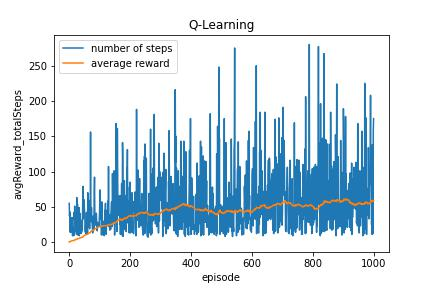
\includegraphics[width=1\linewidth]{q-learning-average-1k.png}
    \caption{Q-Learning Results Over 1000 Episodes}
\end{figure}

Looking at the graph, we can see that the average rewards reached a plateau of approximately 50 after about 200 episodes, this shows that the agent is indeed being trained to
take more optimal actions as the number of episodes increased.

\subsection{Khoi's Progress - SARSA Learning}
The SARSA algorithm is a popular reinforcement learning algorithm. At each time step, the agent selects an action according to its policy, observes the next state and reward, and updates the estimated value of the current state-action pair using a learning rate and discount factor. 
The algorithm maintains a Q-value function that estimates the expected future rewards for each state-action pair. The agent selects an action using an exploration-exploitation strategy and takes the selected action in the environment.

To this end, Khoi is trying to implement an $\epsilon$ greedy method for this SARSA algorithm. He also assumed that the agent will successfully be trained in 1000 episodes. For his setup, the hyperparameters are: $\epsilon = 0.5$; $\gamma = 0.9$; and $\alpha = 0.5$

For the criteria related to the CartPole environment, the agent will play the game for a set number of episodes, and in each episode, the last 100 steps will have their rewards recorded (if the number of steps is less than 100, then the average will be over however many steps was taken for that episode) in order to generate an average.
If any of the failing conditions is met, a penalty of -10 is given, otherwise, a reward of +1 is given. In the plot below, notice that a few episodes have taken around 300 steps, and in general, the average reward stays around the 50 mark.

For one run of 1000 episodes, here are his current results. Note that due to the random nature of taking actions, each run will produce a different graph.

\begin{figure}[H] %h forces the figure to be inserted right here
    \centering
    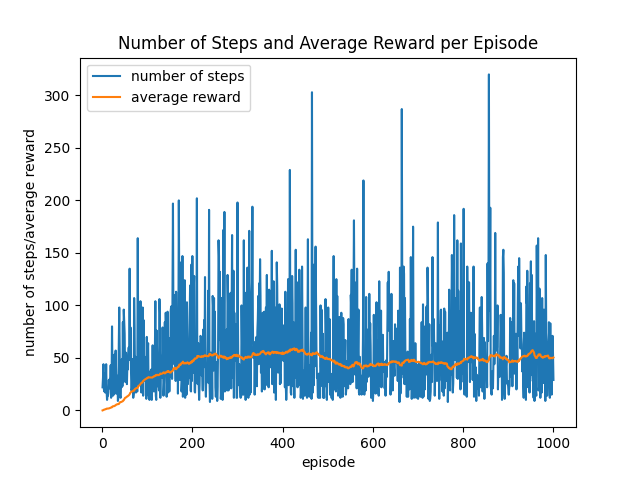
\includegraphics[width=1\linewidth]{sarsa-average-1k.png}
    \caption{SARSA Results Over 1000 Episodes}
\end{figure}

Looking at the graph, we can see that the average rewards reached a plateau of approximately 50 after about 210 to 220 episodes, this shows that the agent is indeed being trained to
take more optimal actions as the number of episodes increased. However, for this run, the reward seems to diverge after 410 episodes, and the average drops down to roughly 48, and remains around
that mark for the rest of the episodes. This could be attributed to the fact that SARSA is using the Q value of the next state, action pair; while Q-Learning uses the maximum expected Q value instead.
If the number of episodes were to be increased, this divergence could be amended.

\section{General Analysis}

The hypothesis was that the algorithms should be able to finish training after 1000 episodes and that SARSA would perform better, but this was not the case.
Looking at the provided graph, we aren't able to conclude if one algorithm is better than the other.
We think that the reason the training didn't finish is that the number of episodes as well as the hyperparameters weren't optimal. 
So in order to rectify this, we plan on increasing the number of total episodes. 
In addition, we are planning to do sensitivity analysis with the hyperparameters and will compare SARSA and Q-Learning further.
In particular, we think the performance might increase if the value of epsilon is higher that allows the agent to take more random actions and explore the action space more effectively.

\section{Difficulties Encountered}

One of the main difficulties we have with this project is figuring out a good way to discretize the state space of the environment.
As such, this hindered our abilities to perform more experiments in a timely manner.
Fortunately, we came across the \textbf{digitize()} function from the \textbf{numpy} package that does the job quite well.

Another issue that we are facing, due to the random nature of picking an action, no two runs are the same. Therefore, conducting some sort of
sensitivity analysis for our hyperparameters has proven to be difficult. We have tried to solve this by setting a seed number at the beginning
of our script, but that does not seem to be an effective solution yet.

Additionally, for both algorithms, the result is unstable. For some runs, the rewards converged to an average of 50-55 after 200 episodes, and remains stable. However, divergence is encountered
as well. This can be seen in the graph of Khoi's SARSA run. Therefore, it was hard to see if the agent was trained well or not.

\section{Future Work}

Our main goal in the next week or so is to finish the training for both algorithms, and then find a way to save it to memory, making it easily recallable in a fresh environment.

Secondly, as mentioned above, we will be doing sensitivity analysis of the hyperparameters; namely $\alpha$, $\gamma$, $\epsilon$ and see how it would
affect our algorithms.

Third, for Khoi's SARSA algorithms, he wants to explore using SARSA($\Lambda$) and compare it to the current SARSA run. 

Fourth, for both algorithms, we will explore different methods for $\epsilon$ decay. Currently, $\epsilon$ is kept at a constant 0.1 for both algorithms.
Exploring $\epsilon$ decay (such as exponential decay) will provide some useful insights for the comparison of the algorithms.

Finally, we want to refine our training to fit our hypothesis of being able to finish training in 1000 episodes and make SARSA outperform Q-Learning.
Additionally, after we have successfully trained the agent, we want to be able to render a video of the game being played; and save the video for presentation purposes.
%\cnote{All written proposals must be no longer than one page per number of people in the group.}

\bibliographystyle{mslapa}
\bibliography{my,book}

\end{document}


% This document was modified from the file originally made available by
% Pat Langley and Andrea Danyluk for ICML-2K. This version was created
% by Iain Murray in 2018, and modified by Alexandre Bouchard in
% 2019 and 2021 and by Csaba Szepesvari, Gang Niu and Sivan Sabato in 2022. 
% Previous contributors include Dan Roy, Lise Getoor and Tobias
% Scheffer, which was slightly modified from the 2010 version by
% Thorsten Joachims & Johannes Fuernkranz, slightly modified from the
% 2009 version by Kiri Wagstaff and Sam Roweis's 2008 version, which is
% slightly modified from Prasad Tadepalli's 2007 version which is a
% lightly changed version of the previous year's version by Andrew
% Moore, which was in turn edited from those of Kristian Kersting and
% Codrina Lauth. Alex Smola contributed to the algorithmic style files.
